\documentclass[12pt]{beamer}
\usepackage[utf8]{inputenc}
\usepackage[T1]{fontenc}
\usetheme{default}
\usecolortheme{beaver}

\begin{document}
	\author{Maomao Wang}
	\title{Two Phase TiAl Polycrystalline}
	\subtitle{Microsctructure Property Enhancement}
	%\logo{}
	\institute{Lanzhou University of Technology}
	%\date{}
	%\subject{}
	%\setbeamercovered{transparent}
	%\setbeamertemplate{navigation symbols}{}
	\begin{frame}[plain]
	\maketitle
\end{frame}

\begin{frame}
\frametitle{Model Creation}
Unite cell of $\rm{TiAl}$ and $\rm{Ti_3Al}$
$\rm{TiAl}$ is \textbf{L10} structure, $\rm{Ti_3Al}$ is \textbf{hcp} structure \textbf{}

\begin{figure}[ht]
	\centering
	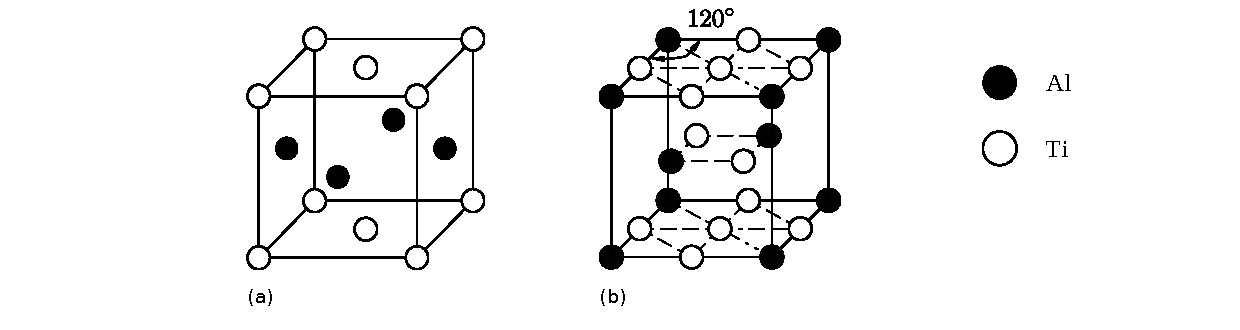
\includegraphics[width=1\linewidth]{img/tial-cell}
	\caption{Unit cell of \rm{TiAl} (a) and $\rm{Ti_3Al}$ (b)}
	\label{fig:tial-cell}
\end{figure}
\end{frame}

\begin{frame}
\frametitle{Model Creation}
Create polycrystalline with and without void defect
\begin{figure}[ht]
	\centering
	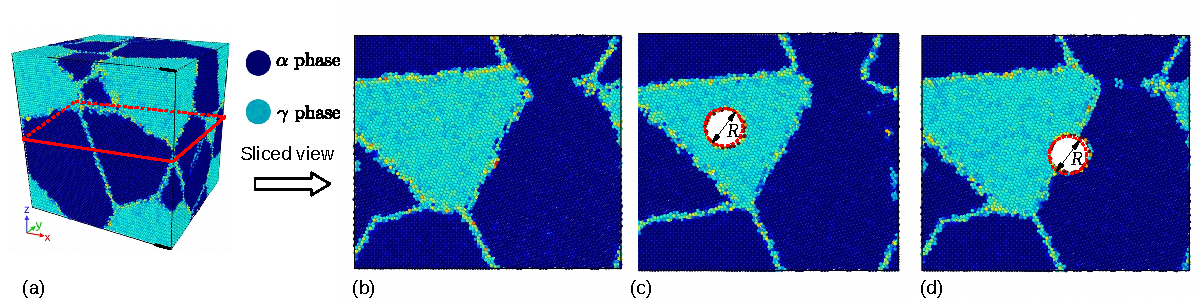
\includegraphics[width=1\linewidth]{img/models}
	\caption{ Model with no void defect (b), with void inside $\alpha_2$ phase (c) with void at $\alpha_2-\gamma$ interface (d)}
	\label{fig:model-creation}
\end{figure}

\end{frame}


\end{document}